\documentclass{article}
\usepackage{graphicx}

\begin{document} 
\begin{center}
{\bf \Large  CMPE 245 Homework 2} \\
\end{center}
Chien-Pin Chen\\
04/13/2015\\

\noindent {\bf Problem 1}. A stochastic process is defined as
\begin{equation}
 x_{k}=x_{k-1}+m_k,\ \ \ x_{0}=0
\end{equation}
where the random variable $m_k$ is defined by the probability density function $p(m_k)$
\begin{equation}
  p(m_{k}) \sim \left\{
    \begin{array}{l}
       0, \ \ \ m_k < -1/2 \\
       4(m_k+1/2), \ \ \ -1/2 \le m_k < 0 \\
       2-4m_k, \ \ \ 0 \le  m_k \le 1/2 \\
       0, \ \ \ \ m_k > 1/2 \\
    \end{array} \right.
\end{equation}
Find the expected value $E\{x_k\}$ and 
the variance $E\{(x_k-\overline{x}_k)^2\}$ of this process.\\ \\
ANS:\\
equation 1. can rewrite as:
\begin{equation}
	\begin{array}{l}
 		x_{k}=x_{k-1}+m_k=x_{k-2}+m_k+m_k=x_{k-2}+2(m_k)\\
 		x_{k}=x_{k-3}+m_k+2(m_k)=x_{k-3}+3(m_k)\\
 		x_{k}=...=x_{0}+k(m_k), \ \ \ where\ x_{0}=0\\
 		x_{k}=k(m_k)
	\end{array}
\end{equation}

Therefore, the expected value can compute as:
\begin{equation}
	\begin{array}{l}
  		E\{x_{k}\}=E\{x_{k-1}+m_k\}=E\{k(m_k)\}=k*E\{m_k\}=k*\int_{-\infty}^\infty m_k\ p(m_k)\ dm_k \\
  		E\{x_{k}\}=k\ \int_{-1/2}^{1/2} m_k\ p(m_k)\ dm_k\\
		E\{x_{k}\}=k\ \int_{-1/2}^{0} m_k\ 4\ (m_k+1/2)\ dm_k+\int_{0}^{1/2} m_k\ (2-4m_k)\ dm_k \\
  		E\{x_{k}\}=k\ (\frac{4}{3}m_k^3+m_k^2 \left| {_{-1/2}^{0} } \right.+\frac{-4}{3}m_k^3+m_k^2 \left| {_{0}^{1/2} } \right.)=k\ \frac{1}{6}\\
	\end{array}
\end{equation}
And, the variance can compute as:
\begin{equation}
	\begin{array}{l}
  		E\{(x_k-\overline{x}_k)^2\}=\int_{-\infty}^\infty (x_k-\overline{x}_k)^2\ p(x)\ dx, \ \ \ where\ x_k=k\ m_k\ and\ \overline{x}_k=E\{x_{k}\}=k\ \frac{1}{6} \\
		E\{(x_k-\overline{x}_k)^2\}=\int_{-\infty}^\infty k\ (m_k-\frac{1}{6})^2\ p(m_k)\ dm_k\\
		E\{(x_k-\overline{x}_k)^2\}=k(\ \int_{-1/2}^{0} (m_k-\frac{1}{6})^2\ 4\ (m_k+1/2)\ dm_k+\int_{0}^{1/2} (m_k-\frac{1}{6})^2\ (2-4m_k)\ dm_k) \\
		E\{(x_k-\overline{x}_k)^2\}=k\ (m_k^4+\frac{2}{9}m_k^3-\frac{5}{18}m_k^2+18m_k \left| {_{-1/2}^{0} } \right.-m_k^4+\frac{10}{9}m_k^3-\frac{7}{18}m_k^2+18m_k \left| {_{0}^{1/2} } \right.)\\
		E\{(x_k-\overline{x}_k)^2\}=k\ \frac{1}{18} \\
	\end{array}
\end{equation}

\noindent {\bf Problem 2} (only for graduate students) It is known that if 
$x$ is a random variable with a pdf $p_x(x)$, i.e., $x \sim p_x(x)$,  
and $y$ is a random variable $y \sim p_y(y)$, then 
$z=x+y$ is a random variable $z \sim p_z(z)$, where $p_z(z)=p_x(x)*p_y(y)$. 
The symbol  $*$ denotes the convolution, i.e.,
\begin{equation}
  p_z(z)=p_z(x+y)=\int_{-\infty}^\infty p_y(z-x)p_x(x)dx
\end{equation}

(a) If $m_k \sim p(m_k)$, where $p(m_k)$ is depicted  in
 the figure, and $m_k=n+h$, figure out $p_n(n)$ and $p_h(h)$.  \\ \\
ANS:\\
Because $m_k=n+h$ and $p_z(z)=p_x(x)*p_y(y)$, I could derive that $p(m_k)=p(n+h)=p_n(n)*p_h(h)$.
$p(m_k)$ is a symmetrical triangular-shaped distribution, and, it is the result of convolution of 
two identical uniform distribution. Therefore, $p_n(n)$ and $p_h(h)$ can be two identical uniform distribution as:
\begin{equation}
  p_n(n) = \left\{
    \begin{array}{l}
       0, \ \ \ n < a \\
       1/(b-a), \ \ \ a \le n \le b \\
       0, \ \ \ \ n > b \\
    \end{array} \right.
    \ \ where\ a=-1/4,\ b=1/4
\end{equation}

(b) Use your conclusion from (a) to write a MATLAB code that
generates the sequence from Problem 1. Generate the sequence 
100 (or more) times and based on these sequences, verify the
results obtained in Problem 1. \\ \\
ANS:\\
First, I use MATLAB to create uniform-shaped function $p_n(n)$ (as figure 1).
Then, I use MATLAB function (conv) to do the convolution of $p_n(n)$ and itself (as figure 2).\\
Finally, I generate the sequence of 100 times $x_k=x_{k-1}+m_k$, and I got $x_k$ about -5 to 5. 
While, according to my result of Problem 1 that $E\{x_k\}=k\ \frac{1}{6}=100*\frac{1}{6}=16.667$.

\begin{figure}
\begin{center}
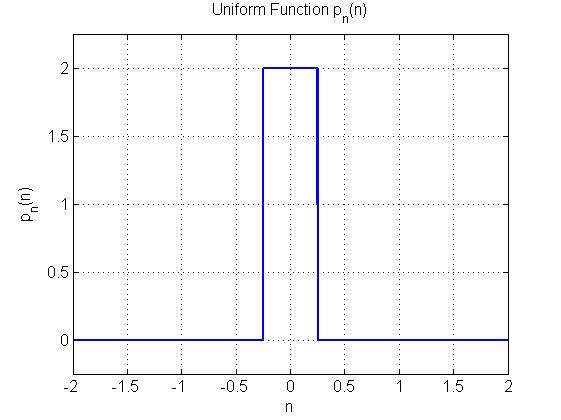
\includegraphics[width=1.0\textwidth]{HW2-1.jpg}
\caption{Uniform Function $ p_n(n) $}
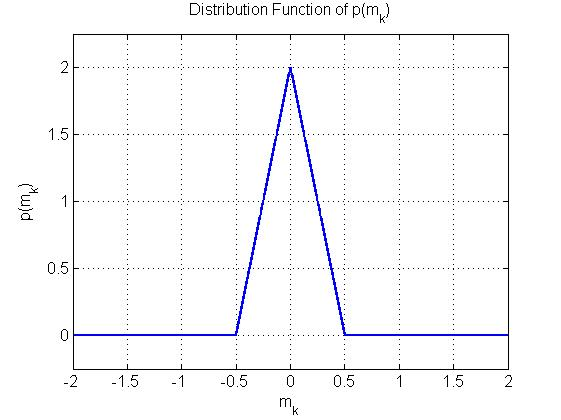
\includegraphics[width=1.0\textwidth]{HW2-2.jpg}
\caption{Distribution Function $ p(m_k) $}
\end{center}
\end{figure}


\end{document}
